%!TEX root = ../Thesis.tex
\section{UserStories \& Use Cases}

% \subsection{User Story}

\subsection*{Niklas Hardes}

Ein Kunde möchte eine persönliche Liste von Spielen anlegen können, mit den für ihn beliebtesten Spielen. Dadurch kann er mit wenig Aufwand diese schnell auf Ihren aktuellen Preis überprüfen. 

\begin{figure}[hbt]
    %\centering
    \begin{minipage}[t]{.7\textwidth} % Breite, z.B. 1\textwidth		
        \caption{Use Case Authentifizieren} % Überschrift
        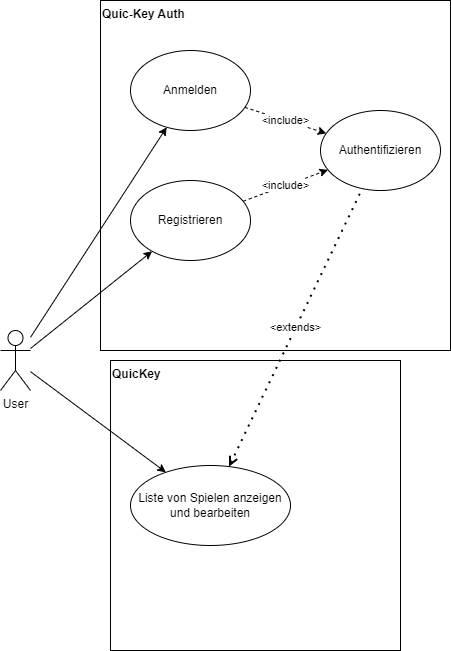
\includegraphics[width=1\textwidth]{img/use_case_auth.png}\\ % Pfad
        \source{Eigene Darstellung} % Quelle
    \end{minipage}
\end{figure}

\subsection*{Robert Hesselmann}

Ein erfolgreicher Streamer auf der Livestreaming Plattform Twitch sucht nach neuen Spielen, die er in seinen Livestreams spielen kann. Um seinen Gewinn zu maximieren sucht er nach einem Spiel zu einem günstigen Preis.

\begin{figure}[hbt]
    %\centering
    \begin{minipage}[t]{.7\textwidth} % Breite, z.B. 1\textwidth		
        \caption{Use Case Streamer} % Überschrift
        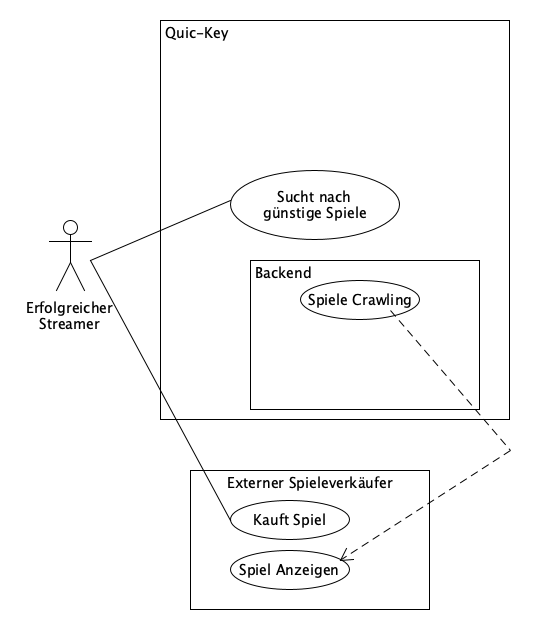
\includegraphics[width=1\textwidth]{img/use_case_streamer.png}\\ % Pfad
        \source{Eigene Darstellung} % Quelle
    \end{minipage}
\end{figure}
    

\subsection*{Nicolas Groß}

Hallo Welt

% \subsection{Use Case}


% \subsubsection*{Robert Hesselmann}



% \subsubsection*{Niklas Hardes}

% \subsubsection*{Nicolas Groß}